\subsection{Mintavételezett jel:}
\begin{figure}[H]
    \centering
    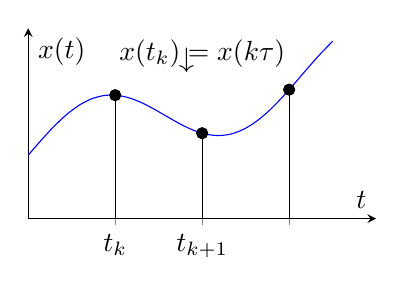
\begin{tikzpicture}[>=latex]
        \begin{axis}[
            axis lines=middle,
            xlabel={$t$}, ylabel={$x(t)$},
            xtick={1, 2, 3}, xticklabels={$t_k$, $t_{k+1}$, {}},
            ytick=\empty,
            ymin=0, ymax=1.5,
            xmin=0, xmax=4,
            width=6cm, height=4cm
        ]
            \addplot[blue, smooth, domain=0:3.5] {0.5 + 0.3*sin(deg(x*2)) + 0.2*x};
            \addplot[ycomb, mark=*, black] coordinates {(1, {0.5 + 0.3*sin(deg(1*2)) + 0.2*1}) (2, {0.5 + 0.3*sin(deg(2*2)) + 0.2*2}) (3, {0.5 + 0.3*sin(deg(3*2)) + 0.2*3})};
            
            \node at (axis cs:2, 1.3) {$x(t_k) = x(k\tau)$};
            \node at (axis cs:1.8, 1.25) [rotate=-90] {$\rightarrow$};
        \end{axis}
    \end{tikzpicture}
    \\
    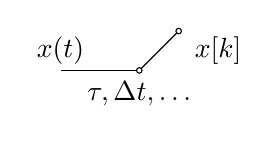
\begin{tikzpicture}
        \draw (0,0) -- (1,0);
        \draw (1,0) -- (1.5, 0.5); 
        \node at (2,0.25) {$x[k]$};
        \node at (0,0.25) {$x(t)$};
        \node at (1, -0.3) {$\tau, \Delta t, \dots$};
        \draw[fill=white] (1,0) circle (1pt);
        \draw[fill=white] (1.5,0.5) circle (1pt);
    \end{tikzpicture}
\end{figure}

\begin{itemize}
    \item a mintavételezés eredményét \textbf{tömbös formában} lehet tárolni:
    \begin{center}
        \begin{tabular}{|c|c|c|c|}
            \hline
            $x(0\tau)$ & $x(1\tau)$ & $x(2\tau)$ & ... \\
            \hline
        \end{tabular}
    \end{center}

    \item ebből matematikai számsorozatot tudunk csinálni:
    $$ \{x_k\} = \{x_0, x_1, x_2, \dots \} $$

    \item állítsunk össze polinomot a sorozat elemeiből:
    $$ a_0 + a_1 x + a_2 x^2 \dots = \sum_{k=0}^N a_k x^k $$

    \item általánosítás: $N \to \infty$ $\rightarrow$ számsorozat $\rightarrow$ sor $\rightarrow$ hatványsor (függvénysor)
    $$ \sum_{k=0}^\infty a_k x^k \to \sum_{k=0}^\infty a_k z^{-k} \to \sum_{k=0}^\infty x[k] z^{-k} =: X(z) $$
    $$ x = z^{-1} \quad \text{Z-transzformáció} $$

    \item cél: $\Delta t = \tau \to 0$
    \begin{itemize}
        \item tudjuk, hogy: $z = e^{\ln(z)}$
        $$ \sum_{k=0}^\infty x(k\tau) z^{-k\frac{\tau}{\tau}} \to \sum_{k=0}^\infty x(k\tau) e^{-\ln(z) k \frac{\tau}{\tau}}, \quad s := \ln(z) / \tau $$
    \end{itemize}

    \item így:
    $$ \sum_{k=0}^\infty x(k\tau) e^{-sk\tau}, \quad k\tau \to t $$

    \item $\tau \to 0 \, (\Delta t \to 0)$:
    $$ \int_0^\infty x(t) e^{-st} dt := X(s) $$
\end{itemize}

\noindent \textbf{Így tehát a Laplace transzformáció:}
$$ F(s) = \mathcal{L}\{f(t)\} = \int_0^\infty f(t) e^{-st} dt $$
\begin{itemize}
    \item $f(t)$ belépő függvény, tehát $t \in [0, \infty) \to f(t)\varepsilon(t)$
\end{itemize}